\documentclass[conference]{IEEEtran}

\usepackage{graphicx}
\usepackage{amsmath,amssymb}
\usepackage{booktabs}
\usepackage{cite}
\usepackage{url}
\usepackage[hidelinks]{hyperref}
\usepackage{xurl}
\usepackage{balance}

\newcommand{\pp}{\,pp}

\title{A ResNet-18 Baseline Study of Distortion-Aware Training for\\
Robust AI-Generated Image Detection}

\author{
\IEEEauthorblockN{Junxuan Cai (Student ID: 521370910086)}
\IEEEauthorblockA{
ECE4880J Computer Vision\\
Global College, Shanghai Jiao Tong University\\
Shanghai, China
}
}

\begin{document}

\maketitle

\begin{abstract}
Routine post-processing is a practical source of distribution shift for
AI-generated image detectors. We measure this shift with two
ImageNet-pretrained ResNet-18 training conditions evaluated across three
seeds. The baseline and distortion-aware conditions use the same 27,643 labeled images
from NTIRE 2026 training shard 5, source-isolated split, optimization schedule,
and evaluation sets. Distortion-aware training adds random JPEG compression, Gaussian
blur, and Gaussian noise during training. Performance is measured on clean
images and five post-processing transformations, using three training seeds,
five severity levels per transformation, and single-component training
comparisons. The baseline obtains $97.30\%$ clean ROC AUC and $94.95\%$ pooled
transformed AUC. Distortion-aware training changes these values to $96.51\%$
and $95.90\%$, respectively: a $0.79\pp$ clean-test reduction, a $0.95\pp$
transformed-test gain, and a $1.74\pp$ reduction in the clean-to-transformed
gap. The direction of this exchange is consistent across seeds. The gain is
concentrated under severe Gaussian noise and blur; JPEG compression and center
crop show no consistent improvement.
\end{abstract}

\begin{IEEEkeywords}
AI-generated image detection, distribution shift, data augmentation,
robustness, image forensics, common corruptions
\end{IEEEkeywords}

\section{Introduction}
\label{sec:introduction}

AI-generated images are commonly recompressed, resized, cropped, or otherwise
edited before they reach a detector. These operations may leave the depicted
content recognizable while weakening low-level traces used for image
forensics. A detector that performs well on original files can therefore lose
accuracy after an image passes through a social platform, messaging service,
or editing tool. Compression, resizing, and blur have consequently become
standard stress tests for synthetic-image detectors
\cite{wang2020cnn,corvi2023diffusion,zhu2023genimage}.

Post-processing robustness is distinct from cross-generator generalization.
The latter asks whether a detector transfers to generators absent from its
training set; the former asks whether a prediction survives changes to the
same source image. This report studies post-processing. The available shard
provides binary real/AI labels but no generator identities, so it does not
support a generator-held-out split. The evaluation therefore covers
source-separated post-processing shifts
\cite{ojha2023universal,yan2025sanity}.

The baseline is an ImageNet-pretrained ResNet-18 trained with
crop, flip, and color augmentation. A second ResNet-18 uses the same images,
split, initialization, loss, optimizer, schedule, model-selection rule, and
test sets, but adds random JPEG compression, Gaussian blur, and Gaussian noise
during training. This isolates the effect of the added distortions without
changing model capacity or training budget. Figure~\ref{fig:pipeline} gives an
overview of the comparison.

The controlled comparison reveals a trade-off: distortion-aware training
improves pooled transformed AUC and narrows the clean-to-transformed gap while
reducing clean AUC. Transformation-specific and severity results locate the
gain mainly in strong noise and blur; JPEG compression and center crop do not
improve consistently.

\begin{figure*}[!t]
    \centering
    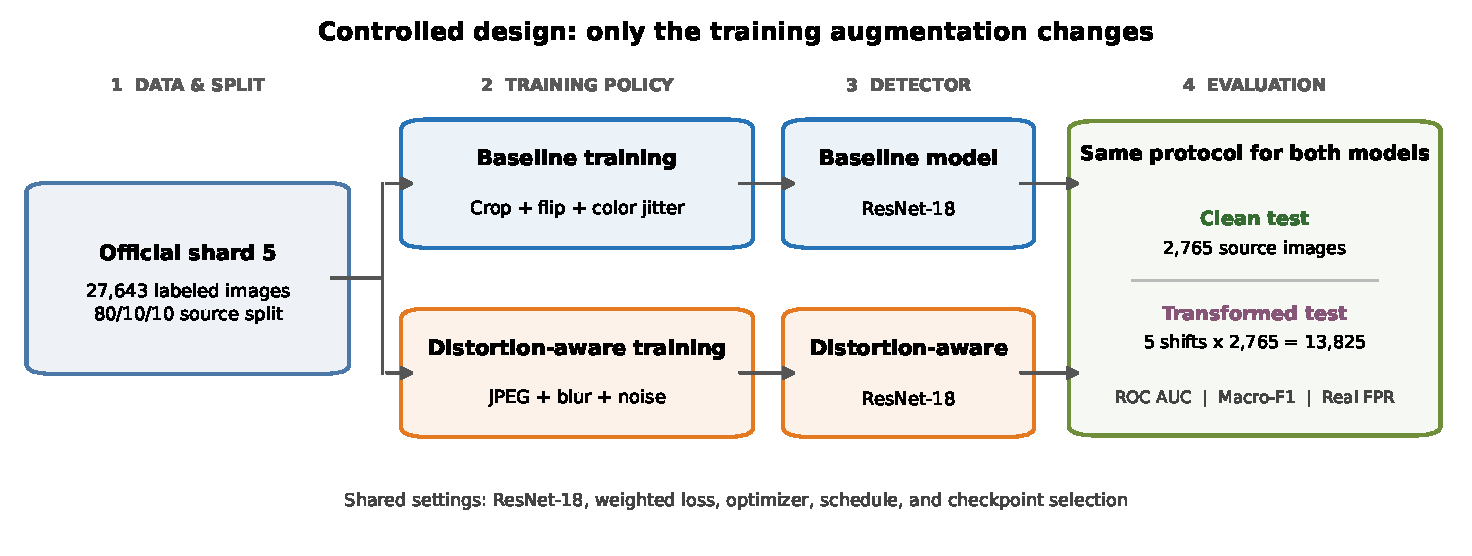
\includegraphics[width=0.98\textwidth]{figures/figure1_experiment_pipeline.pdf}
    \caption{Controlled experiment. Both detectors share the source-image
    split, ResNet-18 architecture, weighted loss, optimizer, schedule, and
    evaluation sets. The baseline uses crop, flip, and color jitter;
    distortion-aware training additionally applies JPEG compression,
    Gaussian blur, and Gaussian noise.}
    \label{fig:pipeline}
\end{figure*}

\section{Related Work}
\label{sec:related_work}

\subsection{Cross-Generator Detection}

Synthetic-image detection has often been studied as transfer from a known
generator to unseen generators. Wang \textit{et al.} trained a binary
classifier on ProGAN samples and found that blur and JPEG augmentation helped
it transfer to several CNN-based generators, although performance remained
generator-dependent \cite{wang2020cnn}. Diffusion models introduced a further
domain change. Corvi \textit{et al.} evaluated GAN-era forensic detectors on
diffusion imagery and included compression and resizing in their analysis
\cite{corvi2023diffusion}; DIRE instead uses the residual between an image and
its diffusion reconstruction as forensic evidence \cite{wang2023dire}.

Recent work has also changed the representation used by the detector. Ojha
\textit{et al.} use fixed features from a large vision-language model to
improve transfer beyond a narrow training domain \cite{ojha2023universal}.
CLIP-based detectors extend this direction with lightweight training and
improved performance on impaired images \cite{cozzolino2024clip}. These
methods address representation and generator transfer. Here, the
representation is held fixed so that changes in robustness can be assigned to
the training distortions.

\subsection{Post-Processing Robustness}

GenImage includes cross-generator tests together with degraded-image
conditions such as low resolution, blur, and compression
\cite{zhu2023genimage}. The full NTIRE 2026 benchmark broadens this setting to
42 generators and 36 transformations and uses ROC AUC on a mixture of
transformed and untransformed images \cite{gushchin2026ntire}. Competitive
systems combine larger training collections, multiple resolutions, strong
augmentation, and heterogeneous backbones; HEDGE is one example
\cite{wu2026hedge}. The present experiment instead uses one official shard and
one compact ResNet-18 to measure the incremental effect of distortion-aware
training against a specified baseline.

The severity sweeps follow the corruption-family evaluation used by
ImageNet-C \cite{hendrycks2019corruptions}. ROC AUC is reported separately
from threshold-dependent metrics because ranking can remain strong even when
a fixed operating threshold is poorly calibrated under shift
\cite{guo2017calibration,ovadia2019uncertainty}.

\section{Dataset and Evaluation Protocol}
\label{sec:dataset}

\subsection{Source Images and Split}

The full NTIRE 2026 benchmark contains 108,750 real images, 185,750 generated
images, 42 generators, and 36 transformations \cite{gushchin2026ntire}. The
experiments use official training shard 5, which contains 27,643 unique JPEG
source images: 9,947 real and 17,696 AI-generated. A stratified 80/10/10 split
with seed 42 assigns 22,113 images to training, 2,765 to validation, and 2,765
to the clean test. Table~\ref{tab:split} lists the class counts.
Transformations are generated only after the source split, and every derived
copy remains in the split of its source image.

\begin{table}[!t]
\centering
\caption{Source-image split used in the experiments.}
\label{tab:split}
\setlength{\tabcolsep}{4.5pt}
\begin{tabular}{lrrr}
\toprule
Split & Real & AI & Total \\
\midrule
Train & 7,957 & 14,156 & 22,113 \\
Validation & 995 & 1,770 & 2,765 \\
Clean test & 995 & 1,770 & 2,765 \\
Transformed test$^{\dagger}$ & 4,975 & 8,850 & 13,825 \\
\bottomrule
\multicolumn{4}{l}{\footnotesize $^{\dagger}$Five transformed copies of every clean-test source.}
\end{tabular}
\end{table}

The shard labels specify only whether an image is real or AI-generated. They
do not identify the generator. The protocol can enforce source separation and
evaluate post-processing shift, but it cannot measure transfer to held-out
generators.

\subsection{Fixed Transformations and Severity Sweeps}

The fixed transformed test is built from the 2,765 clean test sources. Five
operations are applied independently: JPEG compression at quality 35;
Gaussian blur with $\sigma=1.5$; additive Gaussian noise with standard
deviation 0.04 on a $[0,1]$ scale; downsampling to 50\% followed by restoration
to the original dimensions; and a center crop that retains 80\% of the width
and height followed by resizing. The resulting set contains 13,825 images,
five transformed versions of every source, with the original binary labels.
Figure~\ref{fig:shifts} illustrates the five operations on one real and one
AI-generated source.

A separate sweep evaluates five levels for each transformation: JPEG qualities
$\{95,75,55,35,20\}$; blur $\sigma\in\{0.5,1.0,1.5,2.0,3.0\}$; noise standard
deviations $\{0.01,0.02,0.04,0.06,0.08\}$; downsampling factors
$\{0.90,0.75,0.50,0.35,0.25\}$; and retained center-crop fractions
$\{0.95,0.90,0.80,0.70,0.60\}$. Inference then resizes the short side to 256
pixels, takes a $224\times224$ center crop, and applies ImageNet normalization.
For the fixed transformed test, non-JPEG outputs are saved once at JPEG quality
95, while the JPEG condition is saved at quality 35. Severity transformations
are applied in memory during evaluation. Two training policies, three seeds,
five transformation families, and five levels produce 150 severity conditions.

\section{Method}
\label{sec:method}

\subsection{ResNet-18 Baseline}

Both conditions use an ImageNet-pretrained ResNet-18 \cite{he2016resnet}. For
an input $x_i$ with label $y_i\in\{0,1\}$, the network produces
$p_\theta(y\mid x_i)$. Its 512-dimensional global-average-pooled feature is
passed through dropout with probability 0.20 and a two-output linear layer.
All backbone parameters are fine-tuned at $224\times224$ resolution. Training
uses weighted cross entropy,
\begin{equation}
\mathcal{L}(\theta)=-\frac{1}{N}\sum_{i=1}^{N}w_{y_i}
\log p_\theta(y_i\mid T(x_i)),
\label{eq:loss}
\end{equation}
with $w_{\mathrm{real}}=1.389531$ and
$w_{\mathrm{AI}}=0.781047$.

The baseline policy applies
RandomResizedCrop with scale 0.7--1.0 and aspect ratio 0.8--1.25, horizontal
flipping, and ColorJitter with brightness 0.15, contrast 0.15, saturation
0.10, and hue 0.03, followed by ImageNet normalization.

\subsection{Distortion-Aware Training}

The distortion-aware policy retains every baseline operation and adds three
stochastic transformations. JPEG compression is applied with probability
0.35 at a quality sampled from 35--95. Gaussian blur is applied with
probability 0.25 and $\sigma\in[0.1,2.0]$. Gaussian noise is applied with
probability 0.20 and a standard deviation sampled up to 0.04. This is the only
difference between the two main training conditions.
Table~\ref{tab:config} summarizes the controlled comparison.

\begin{table*}[!t]
\centering
\caption{Controlled training configuration. Entries marked ``same'' are
identical to the baseline.}
\label{tab:config}
\setlength{\tabcolsep}{5pt}
\begin{tabular}{lll}
\toprule
Component & Baseline & Distortion-aware training \\
\midrule
Backbone and input & ImageNet ResNet-18, $224\times224$ & Same \\
Head and objective & Dropout 0.20, linear head, weighted cross entropy & Same \\
Common augmentation & Crop, flip, color jitter & Same \\
Added distortions & None & JPEG ($p=0.35$), blur ($p=0.25$), noise ($p=0.20$) \\
Optimization & AdamW, batch 32, 10 epochs, warm-up + cosine decay & Same \\
Model selection & Highest validation ROC AUC & Same \\
\bottomrule
\end{tabular}
\end{table*}

Both conditions are optimized for 10 epochs with AdamW
\cite{loshchilov2019adamw}, batch size 32, learning rate $10^{-4}$, weight
decay $10^{-4}$, one warm-up epoch, cosine decay to 1\% of the initial learning
rate, and mixed-precision training. The checkpoint with the highest validation
ROC AUC is retained. The complete comparison is repeated with seeds 42, 43,
and 44.

\section{Experiments and Results}
\label{sec:results}

\subsection{Metrics and Reproducibility}

ROC AUC is the primary metric because it evaluates score ranking over all
thresholds and matches the NTIRE challenge metric \cite{gushchin2026ntire}.
Macro-F1 weights the real and AI classes equally. Real-image false-positive
rate (FPR) records the proportion of authentic images classified as AI. For
each checkpoint, a decision threshold is selected on the validation set by
maximizing Youden's statistic $J=\mathrm{TPR}-\mathrm{FPR}$ and is then held
fixed for the clean and transformed tests.

The robustness gap is
\begin{equation}
G=100\,(\mathrm{AUC}_{\mathrm{clean}}-
\mathrm{AUC}_{\mathrm{transformed}}),
\label{eq:gap}
\end{equation}
in percentage points. The pooled transformed AUC is computed over all 13,825
transformed instances; it is not the arithmetic mean of the five
transformation-specific AUCs. We report the mean and sample standard deviation
over three seeds. For the seed-42 model pair, 2,000 paired bootstrap resamples
are drawn at the source-image level \cite{efron1979bootstrap}, keeping the five
transformed copies of each source together.

Training and evaluation used PyTorch 2.13.0 with CUDA 13.0 on an NVIDIA RTX
5070 Ti with 16 GB VRAM, an AMD Ryzen 7 9800X3D, and 32 GB system memory.
Seed-matched runs use identical manifests, initial pretraining, optimizer
settings, schedules, and checkpoint rules.

\subsection{Baseline Degradation and Main Comparison}

Table~\ref{tab:main} reports the three-seed comparison. The baseline reaches
$97.30\%$ clean AUC and $94.95\%$ pooled transformed AUC, a drop of
$2.35\pp$. Its transformed Macro-F1 is $87.20\%$, and $12.72\%$ of real
transformed images cross the validation-selected threshold.

Distortion-aware training reaches $96.51\%$ clean AUC and $95.90\%$
transformed AUC. Relative to the baseline, clean AUC decreases by $0.79\pp$,
transformed AUC increases by $0.95\pp$, and the robustness gap falls by
$1.74\pp$ to $0.61\pp$. Transformed Macro-F1 rises by $1.33\pp$, while real-image FPR falls
by $1.44\pp$.

\begin{table*}[!t]
\centering
\caption{Baseline and distortion-aware results on the clean and pooled
transformed tests (mean $\pm$ sample standard deviation over seeds 42, 43,
and 44, in percent).}
\label{tab:main}
\setlength{\tabcolsep}{7pt}
\begin{tabular}{lccccc}
\toprule
Training & Clean AUC $\uparrow$ & Trans. AUC $\uparrow$ & AUC gap $\downarrow$ &
Trans. Macro-F1 $\uparrow$ & Trans. real FPR $\downarrow$ \\
\midrule
Baseline & \textbf{97.30 $\pm$ 0.11} & 94.95 $\pm$ 0.26 & 2.35 $\pm$ 0.20 &
87.20 $\pm$ 0.72 & 12.72 $\pm$ 0.37 \\
Distortion-aware & 96.51 $\pm$ 0.26 & \textbf{95.90 $\pm$ 0.26} &
\textbf{0.61 $\pm$ 0.03} & \textbf{88.54 $\pm$ 0.46} &
\textbf{11.28 $\pm$ 0.46} \\
\bottomrule
\end{tabular}
\end{table*}

Figure~\ref{fig:main-effect} reports the seed-42 paired bootstrap comparison.
The 95\% intervals exclude zero for all three contrasts: clean AUC
$-1.03\pp$ (95\% CI $[-1.52,-0.58]$), transformed AUC $+0.91\pp$
($[+0.40,+1.40]$), and gap reduction $+1.94\pp$
($[+1.70,+2.20]$). Figure~\ref{fig:seeds} reports the seed-matched effects for
all three training runs. Each seed records lower clean AUC, higher transformed
AUC, and a smaller robustness gap after distortion-aware training.

\begin{figure*}[!t]
    \centering
    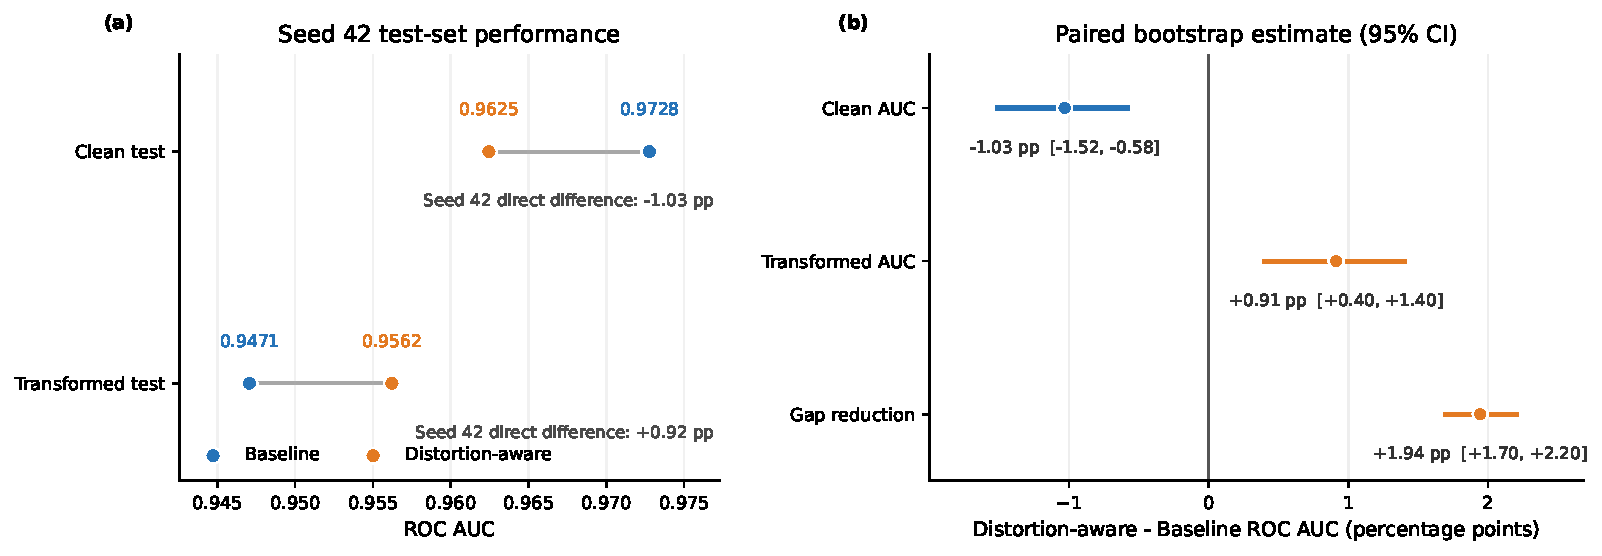
\includegraphics[width=0.84\textwidth]{figures/figure4_effect_sizes_and_stability.pdf}
    \caption{Seed-42 paired comparison. The left panel compares baseline and
    distortion-aware AUC on the clean and transformed tests; gray segments
    show the within-test difference. The right panel reports
    distortion-aware-minus-baseline effects; bars are 95\% source-level
    paired-bootstrap confidence intervals.}
    \label{fig:main-effect}
\end{figure*}

\begin{figure*}[!t]
    \centering
    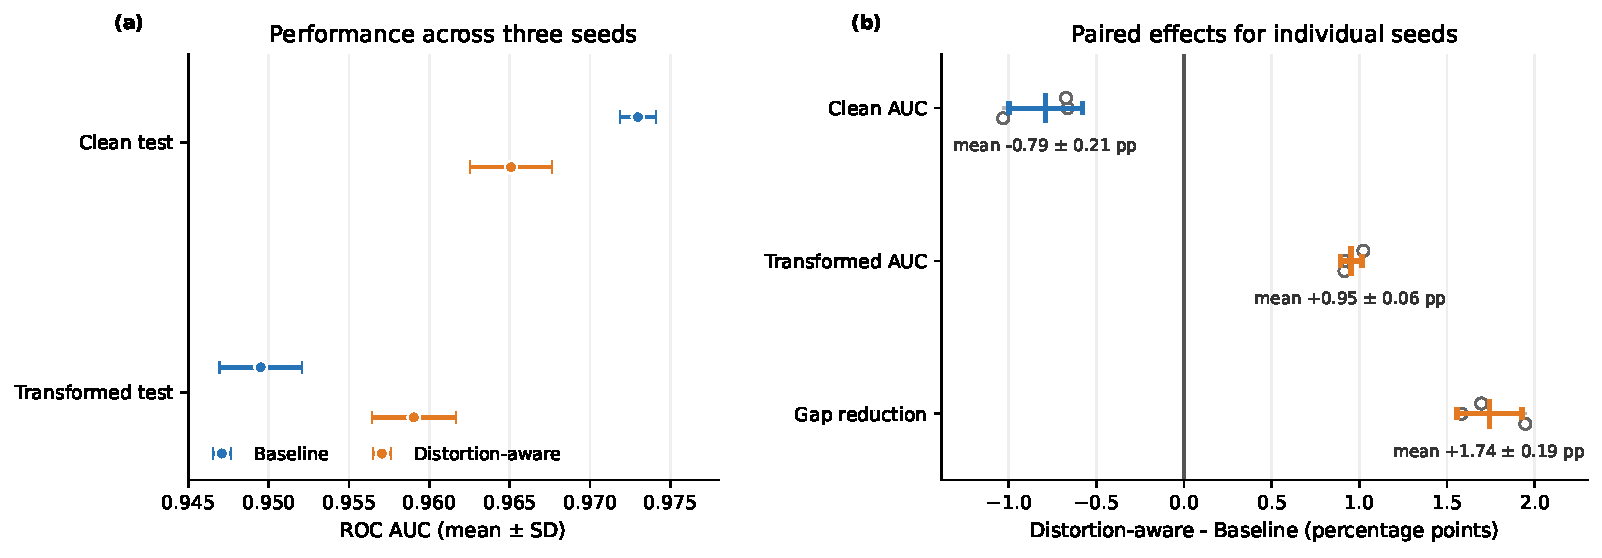
\includegraphics[width=0.82\textwidth]{figures/figure8_seed_variability.pdf}
    \caption{Three-seed stability. Panel (a) reports absolute clean and
    transformed AUC as the mean and one sample standard deviation. Panel (b)
    shows individual seed-matched effects together with their mean and sample
    standard deviation. Positive transformed-AUC and gap-reduction values
    favor distortion-aware training.}
    \label{fig:seeds}
\end{figure*}

\subsection{Results by Transformation}

The pooled improvement is not uniform across transformations.
Figure~\ref{fig:per-transform} reports distortion-aware minus baseline effects
over three seeds. Blur AUC changes by $+0.04\pp$, while blur Macro-F1 rises
$1.36\pp$ and its real-image FPR falls $11.66\pp$. Noise gains $0.75\pp$ AUC
and $7.12\pp$ Macro-F1, although its real-image FPR increases by $6.37\pp$.
Downsampling AUC changes by $-0.23\pp$ while real-image FPR improves by $6.97\pp$.
Center crop and JPEG lose $0.97\pp$ and $0.65\pp$ AUC, respectively.

\begin{figure*}[!t]
    \centering
    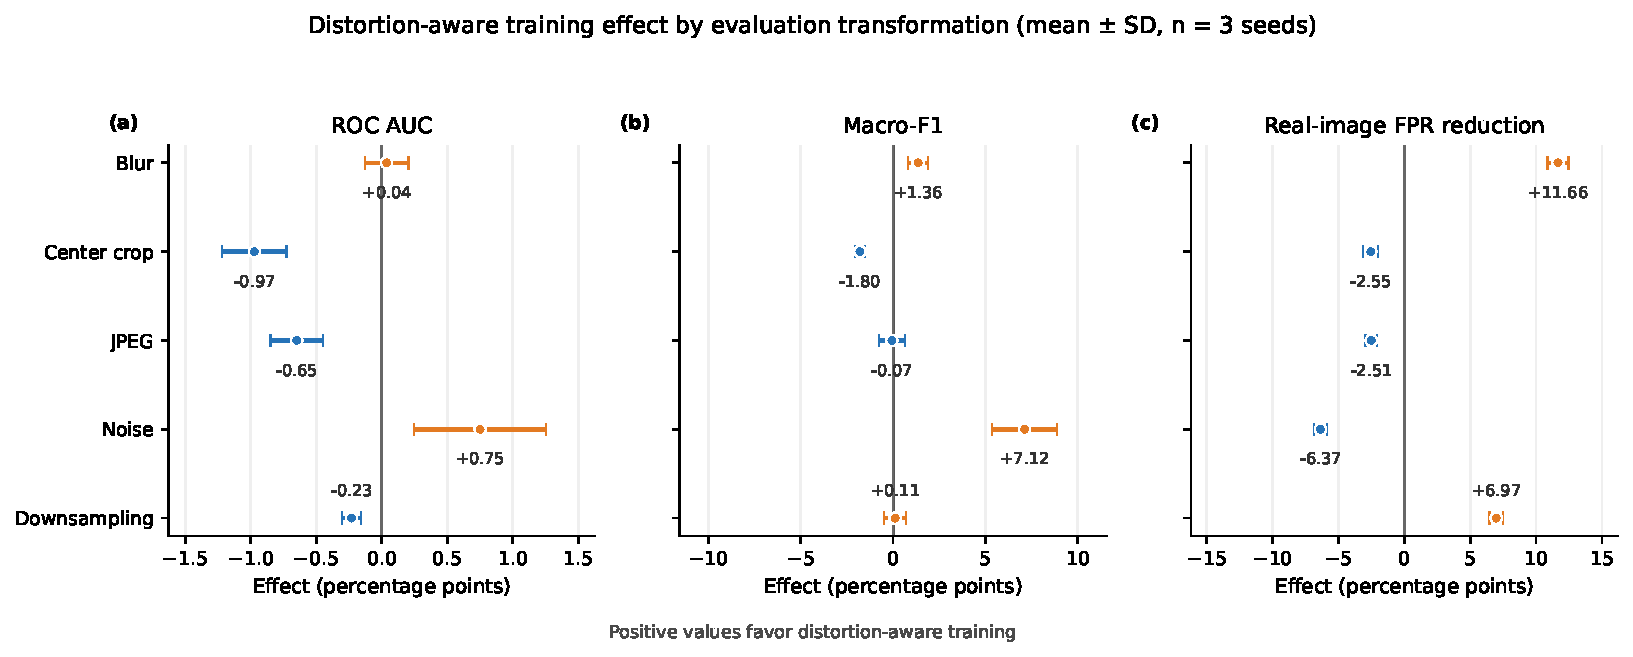
\includegraphics[width=0.83\textwidth]{figures/figure12_per_transformation_effect_heatmap.pdf}
    \caption{Change from baseline by transformation, averaged over three
    seeds. Columns report ROC AUC, Macro-F1, and real-image FPR reduction in
    percentage points; points are means and bars show one sample standard
    deviation. Positive values favor distortion-aware training.}
    \label{fig:per-transform}
\end{figure*}

Pooled ROC AUC ranks all 13,825 transformed instances jointly and therefore
also reflects score ordering across transformation families. The separate
scores in Fig.~\ref{fig:per-transform} locate the conditions that contribute
to, or work against, the pooled result.

\subsection{Severity Response}

Figure~\ref{fig:severity} follows each transformation from mild to severe.
The distortion-aware advantage grows most strongly under Gaussian noise. At
the highest tested noise level, AUC is $95.08\%$ versus $90.40\%$ for the
baseline, a $4.68\pp$ gain. The strongest blur and downsampling conditions
gain $1.30\pp$ and $0.67\pp$, respectively. Averaged over the five levels,
the effects are $+1.56\pp$ for noise, $+0.06\pp$ for blur, and $-0.21\pp$ for
downsampling. JPEG and crop remain negative on average ($-0.63\pp$ and
$-0.84\pp$).

\begin{figure*}[!t]
    \centering
    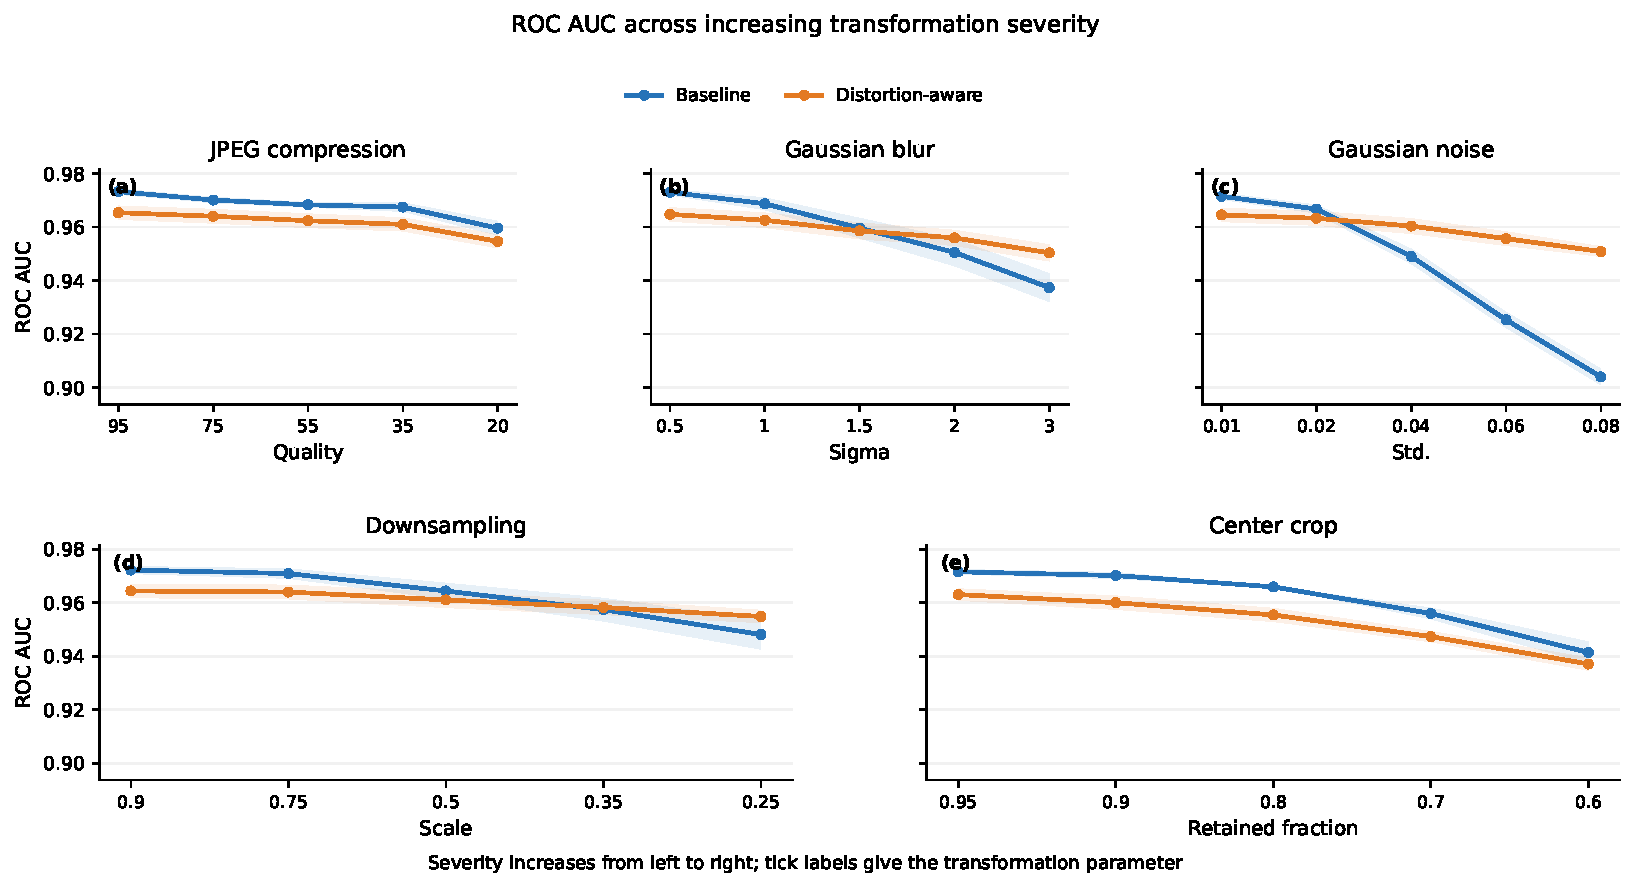
\includegraphics[width=0.88\textwidth]{figures/figure13_severity_auc_curves.pdf}
    \caption{ROC AUC for the baseline and distortion-aware model over five
    severity levels. Lines are three-seed means, and bands show one sample
    standard deviation. Severity increases from left to right.}
    \label{fig:severity}
\end{figure*}

The advantage is concentrated at high noise and blur severity. Exposure to a
transformation during training is not sufficient by itself: the JPEG policy
does not improve the JPEG sweep, and center crop remains a failure mode.
Downsampling was absent from the three added distortions, yet records a small
gain at the strongest level, which suggests limited transfer across
distortion families.

\begin{figure*}[!t]
    \centering
    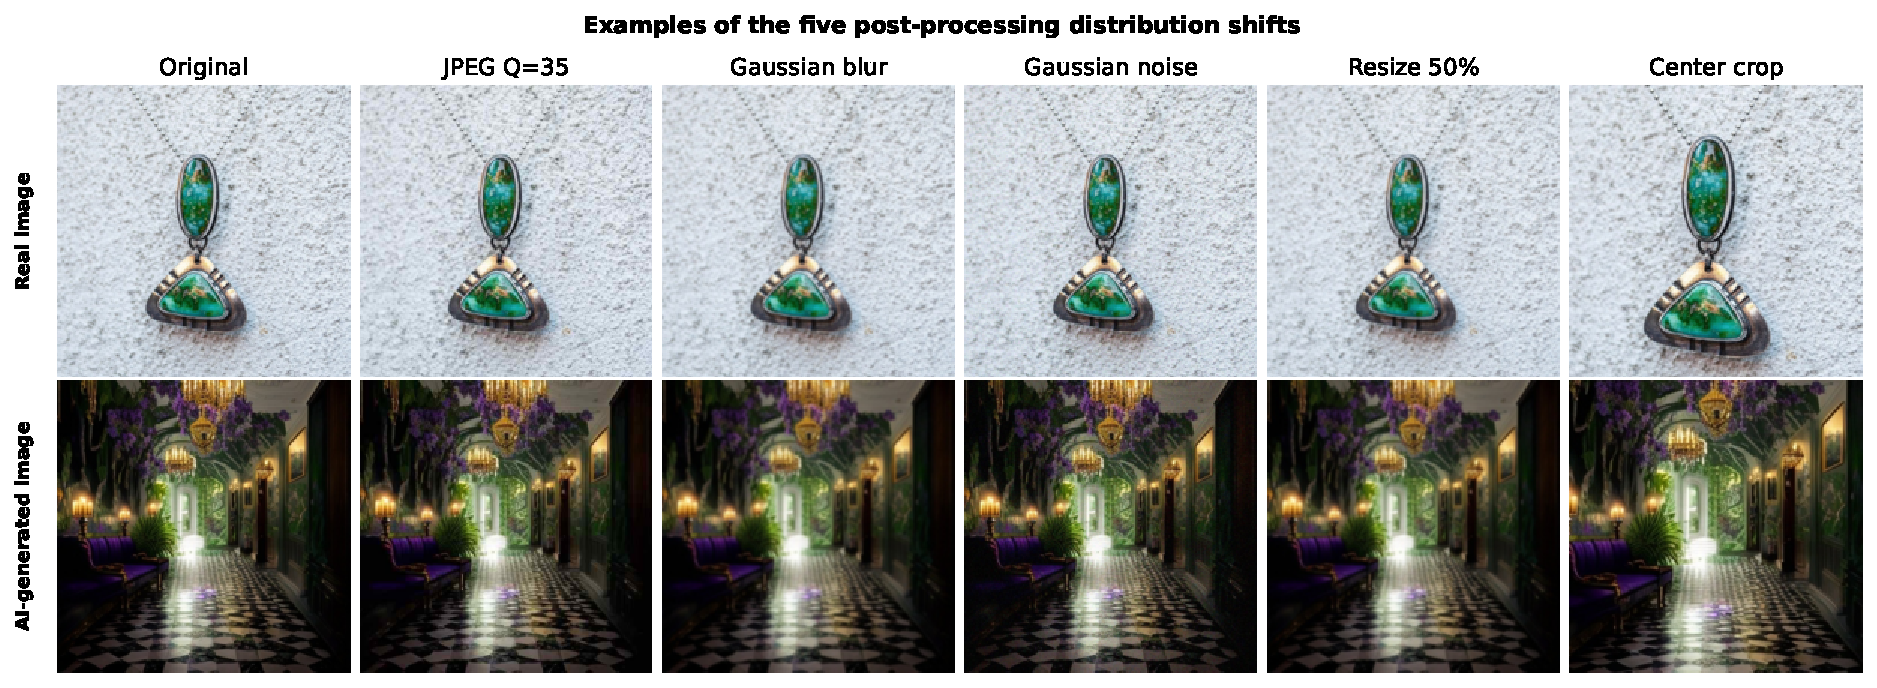
\includegraphics[width=0.90\textwidth]{figures/figure2_transformation_examples.pdf}
    \caption{Two held-out sources before and after the five fixed
    post-processing operations. Each row preserves source identity and class
    label.}
    \label{fig:shifts}
\end{figure*}

\subsection{Exploratory Single-Component Comparison}

The seed-42 comparison in Table~\ref{tab:ablation} replaces the combined
policy with JPEG-only, blur-only, or noise-only training. All three
single-component policies improve pooled transformed AUC relative to the
baseline. Blur-only records the highest transformed AUC ($95.93\%$) and the
lowest real-image FPR ($9.71\%$) on this seed. Noise-only reaches $95.83\%$
transformed AUC but also the highest real-image FPR ($15.98\%$). The combined
policy has the smallest clean-to-transformed gap ($0.62\pp$). Because this
comparison uses one seed, its role is descriptive.

\begin{table}[!t]
\centering
\caption{Single-component training comparison for seed 42 (percent).}
\label{tab:ablation}
\setlength{\tabcolsep}{3.2pt}
\begin{tabular}{lrrrr}
\toprule
Training & Clean & Trans. & Gap & Real FPR \\
\midrule
Baseline & \textbf{97.28} & 94.71 & 2.57 & 12.50 \\
JPEG only & 97.05 & 95.24 & 1.82 & 11.02 \\
Blur only & 97.18 & \textbf{95.93} & 1.26 & \textbf{9.71} \\
Noise only & 97.14 & 95.83 & 1.31 & 15.98 \\
Combined & 96.25 & 95.62 & \textbf{0.62} & 10.87 \\
\bottomrule
\end{tabular}
\end{table}

\section{Discussion}
\label{sec:discussion}

The baseline quantifies the effect of routine post-processing on score
ranking. Distortion-aware training recovers part of the transformed-set
performance, but the exchange is asymmetric across input conditions. A mostly
pristine stream favors the baseline's clean ranking, while a stream containing
strong noise or blur places more value on distortion-aware training.

Ranking and threshold metrics describe different aspects of the model. Under
noise, distortion-aware training improves AUC and Macro-F1 while increasing
the proportion of real images that cross the fixed threshold. Under blur, AUC
changes little while real-image FPR falls markedly. ROC AUC measures ordering
over all thresholds, whereas FPR is tied to one operating point. Deployment
would require a threshold selected for the expected class balance and the
relative costs of false accusations and missed synthetic images.

Grad-CAM \cite{selvaraju2017gradcam} provides a qualitative diagnostic in
Fig.~\ref{fig:gradcam}. In panel (a), distortion-aware training corrects a
blurred real image that the baseline assigns to the AI class. In panel (b), it
introduces the opposite error on a cropped AI image. In these examples, the
attribution maps differ between checkpoints, consistent with a change in the
spatial evidence used for prediction. These maps are case-level diagnostics;
the quantitative comparisons above provide the evidence for performance.

\begin{figure}[!t]
    \centering
    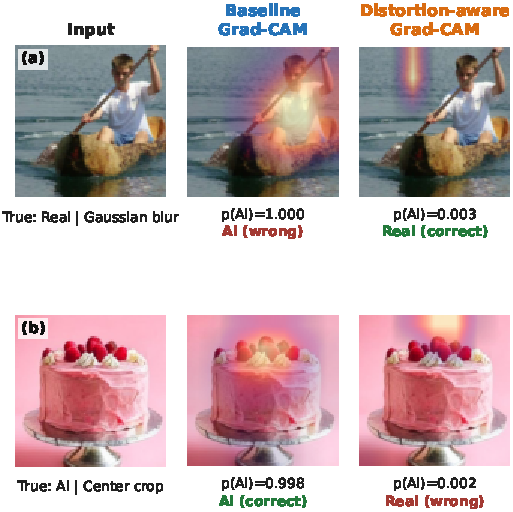
\includegraphics[width=0.98\columnwidth]{figures/figure17_gradcam_comparison.pdf}
    \caption{Seed-42 Grad-CAM maps for two predictions changed by
    distortion-aware training: (a) a blurred real image corrected by the
    model and (b) a cropped AI image newly misclassified as real. Warmer
    regions indicate stronger spatial evidence.}
    \label{fig:gradcam}
\end{figure}

\section{Limitations}
\label{sec:limitations}

The study covers 27,643 source images from one of the six official training
shards. Its content distribution may differ from the remaining shards and
from images encountered after deployment. Generator
identities are absent from the labels used here. The results measure
post-processing robustness for a source-separated binary split, while a
temporal benchmark such as AI-GenBench is designed to study future generators
\cite{pellegrini2025aigenbench}.

The comparison uses one ResNet-18 at $224\times224$. Higher-resolution inputs,
CLIP features, or heterogeneous ensembles may respond differently to the same
augmentation policy \cite{cozzolino2024clip,wu2026hedge}. Each transformed test
image also contains one synthetic operation, whereas platform pipelines may
apply several operations in sequence and introduce codec, content, and format
biases. Challenging-set studies similarly show that benchmark accuracy does
not determine open-world reliability \cite{yan2025sanity}.

The main baseline-versus-combined comparison uses three seeds, but the
component analysis and Grad-CAM examples use seed 42 only. The evidence in
this report is therefore strongest for the three-seed AUC, Macro-F1, FPR, and
severity comparisons on NTIRE 2026 shard 5.

\section{Conclusion}
\label{sec:conclusion}

The ResNet-18 baseline achieved $97.30\%$ clean AUC and $94.95\%$ pooled
transformed AUC on NTIRE 2026 shard 5. Adding JPEG compression, Gaussian blur,
and Gaussian noise to the same training pipeline changed these values to
$96.51\%$ and $95.90\%$. Across three seeds, distortion-aware training exchanged
$0.79\pp$ of clean AUC for a $0.95\pp$ transformed-AUC gain and a $1.74\pp$
reduction in the clean-to-transformed gap. The improvement was largest under
severe noise and blur; JPEG compression and center crop did not improve
consistently. For this model and shard, distortion-aware training is most
useful when the expected input stream contains the severe noise and blur
conditions for which gains were observed. Evaluation across generator-aware
splits, additional backbones, and composed platform processing is the next
step.

\balance
\bibliographystyle{IEEEtran}
\bibliography{references}

\end{document}
